\documentclass[UTF8]{ctexart}
\usepackage{bookmark}
\usepackage{geometry}
\usepackage{hyperref}
\geometry{a4paper,scale=0.8}
\usepackage{ctex}
\usepackage{booktabs}
\usepackage{array}
\usepackage{fancyhdr}
\usepackage{physics}
\pagestyle{fancy}
\fancyhf{}
\renewcommand\footrulewidth{1pt}
\lhead{\textit{王铠泽}}
\rhead{\textit{PB18020766}}
\chead{\href{mailto:volar@mail.ustc.edu.cn}{\textit{volar@mail.ustc.edu.cn}}}
\rfoot{\href{http://en.ustc.edu.cn/}{\textit{中国科学技术大学}}}
\lfoot{\textit{\today}}
\usepackage{graphicx}
\usepackage{float}
\usepackage{subfigure}
\fancyfoot[C]{\textit{\thepage}}


\begin{document}

	\centering\textbf{\LARGE{计算物理A第十八次作业}}
	
	
	\textit{王铠泽\qquad PB18020766}
	
		
	\section{作业题目}
	
	\begin{itemize}
		\item 进行单中心DLA模型的模拟(可以用圆形边界,也可
		以用正方形边界),并用两种方法计算模拟得到的DLA图形的分
		形维数,求分形维数时需要作出双对数图。
	\end{itemize}
	
	\section{实现方法}
	
	\begin{itemize}
		\item DLA生长摸拟
		
		$DLA$的想法是存在若干生长中心,外界的粒子从边界上生成并且进行随机游走,若触碰到生长中心,则停下游走形成团簇,后续的粒子若碰到团簇就被粘住,形成一个生长的图案。
		
		本次实验中采取的算法如下:
		
		建立$(N+1)\times (N+1)$背景网格,使用二维数组 $cnt[N+1][N+1]$来记录生长情况。生长中心的对称中心定在$cnt[N/2][N/2]$。程序初始化时,$cnt$数组全部置零(表示未生长),然后给一个$(2d+1)\times(2d+1)$大小的生长中心赋值为1,表示此处是生长的核。接下来,不断随机地从边界生成粒子,让粒子随机游走,判断是否游走出边界,若走出边界,则开始新粒子的进入,若下一步就会和值为1的矩阵元素重合,则此处也将矩阵元素从0变为1,表示粒子生长到此处。调节模拟中投入的粒子总数$NP$得到不同尺寸的DLA图案。本次实验设置$N=400$,$d=1$,$NP=10^6$,运行时长较长。
		
		\item sandbox计数法
		
		sandbox法是一种很好的计算单中心生长的分形维数的方法。其原理是计算一系列边长为$r$的盒子中的生长粒子个数$N$。理论上,对于分形图形,有$N(r)\sim r^D$。做出双对数图,可以通过直线斜率求得分形维数$D$。
		
		本次实验中采取的算法如下:
		
		在得到生长矩阵$cnt$之后,采用从中心$cnt[N/2][N/2]$开始往外计数的方法,以步长为1开始计数并将每一步对应的数据输入txt文件,直到将包裹这个图形的最小方形给计数完毕就退出循环。
		
		\item 回转半径法($R_g$法)
		
		回转半径法也是一种计算自相似图形分形维数的方法。计算回转半径公式如下:
		
		$$R_g^2=\frac{\sum_{i=1}^N r_i^2}{N}$$
		
		根据计数的个数(面积)$N$和$R_g$满足$N\sim R_g^D$来得到分形维数。
		
		本次实验中采取的算法如下:
		
		在得到生长矩阵之后,开始和sandbox法一样从中心开始一层一层计数,计数得到的个数为$N$,同时在计数过程中可以计算得到不同$N$下的回转半径$R_g$。最后将各个数据输出到txt文件中。 值得一提的是为了避免生长的边缘效应造成的误差,我将输出控制在计数的粒子数为总生长的0.7。
	\end{itemize}
	
	\section{程式说明}
	
	\begin{itemize}
	\item DLA.c
	
	这是一个用于生成$DLA$点阵上的生长与否信息的文件的程式。同时具有输出两种计算分形维数方法相关的数据的功能。
	
	
	\item rdm.h

	这是一个包含了使用16807产生器生成指定长度的$[0,1]$上均匀分布随机数函数的头文件。

	\subitem double rdm()

	该函数输出值为(0,1)上的随机数,生成的方法是线性同余法,具体是16807生成器实现。使用的初始种子为$I$=46984,然后每一次能采用静态变量的方法记录$I_n$的值,实现每一次输出值都不同的效果。
	
	\item size\_(N+1)\_(\# of particles).txt
	
	这是输出背景矩阵为(N+1)$\times$(N+1)维,总共生长粒子数为(\# of particles)的数据txt文件。
	
	\item sandbox.txt
	
	这是输出盒子边长$r$(第一列)和像素计数$N$的数据文件。
	
	\item Rg.txt
	
	这是输出面积(第一列)和回转半径$R_g$的数据文件。
	

	\end{itemize}
	
	
		
	
	\section{计算结果}
	
	\subsection{$DLA$生长图示}
	
	\begin{flushleft}
		采取背景网格为401$\times$401,不同生长阶段图解如下:
		
		\begin{figure}[H]
					\centering  %图片全局居中
					\subfigure[751 particles]{
						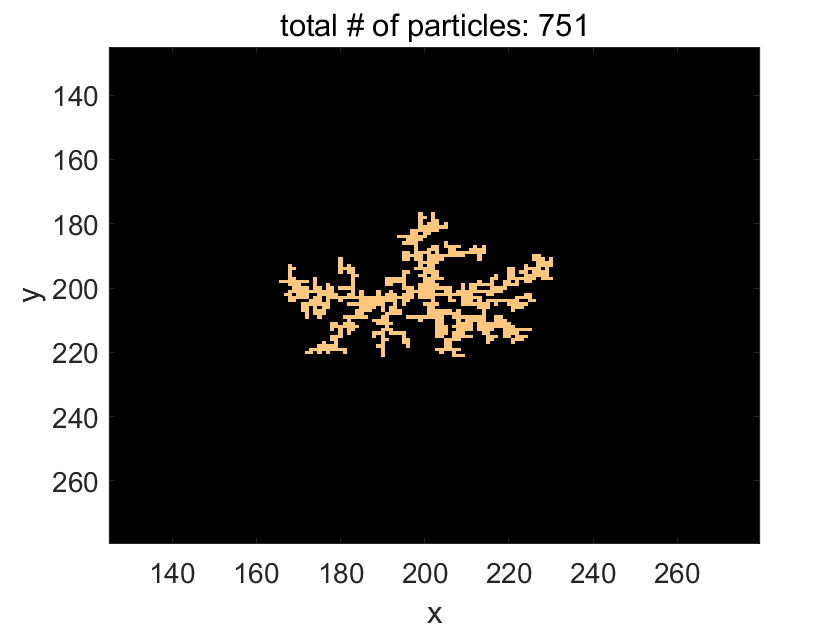
\includegraphics[width=0.45\textwidth]{../result/401_751}}
					\subfigure[1801 particles]{
						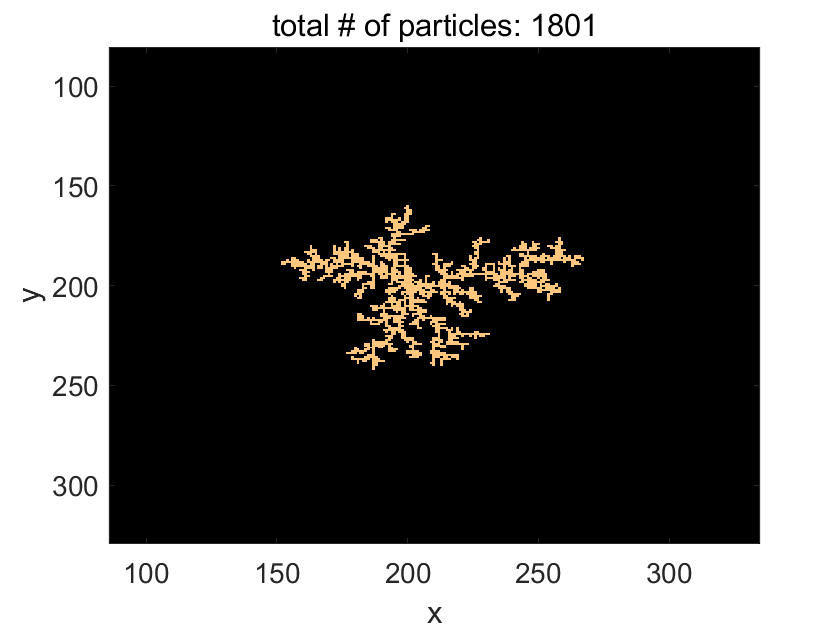
\includegraphics[width=0.45\textwidth]{../result/401_1801}}
					\subfigure[4668 particles]{
						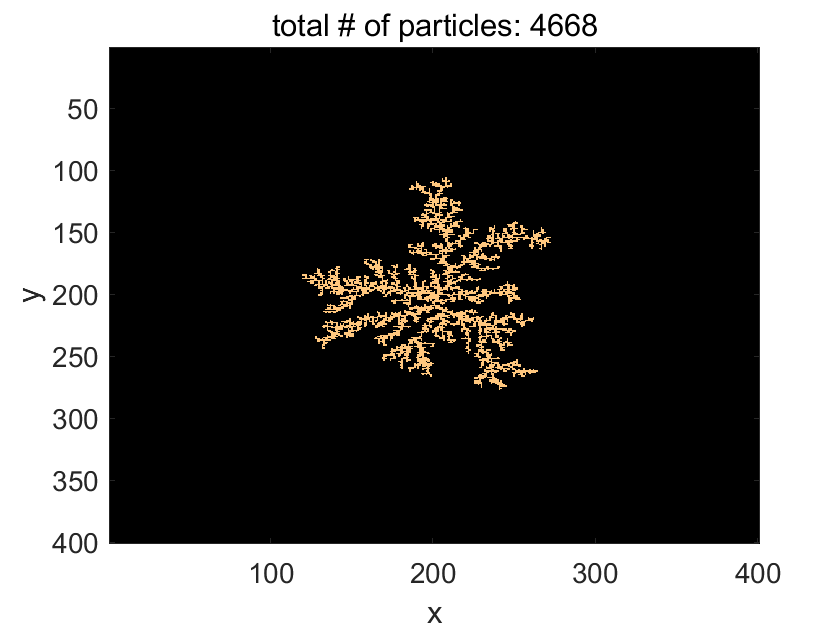
\includegraphics[width=0.45\textwidth]{../result/401_4668}}
					\subfigure[9431 particles]{
						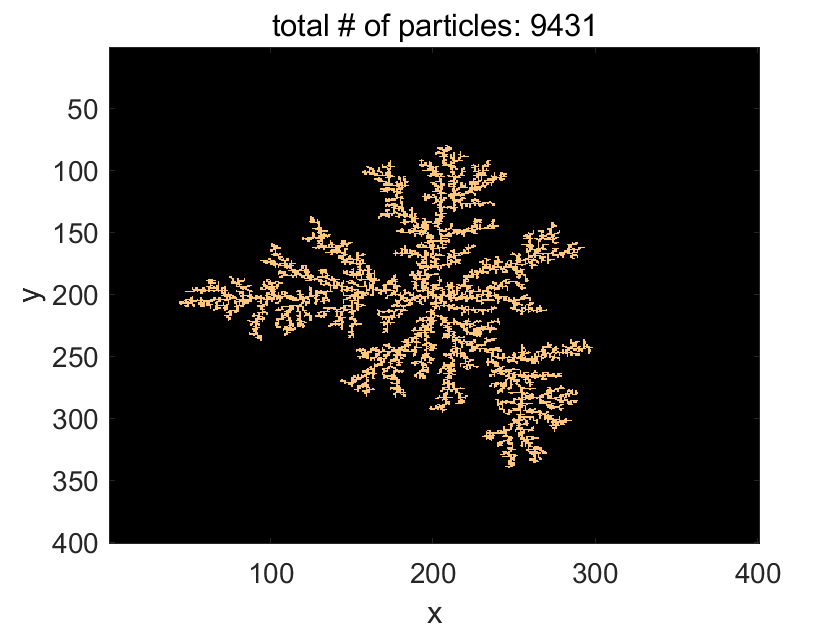
\includegraphics[width=0.45\textwidth]{../result/401_9431}}
					
					\caption{不同阶段的DLA生长}
		\end{figure}
	
	可以看出粒子清晰地体现出延展方向,呈支状生长。
	
	笔者还尝试了二中心的生长情况:
	
		\begin{figure}[H]
		\centering  %图片全局居中
		\subfigure[751 particles(中心相距远)]{
			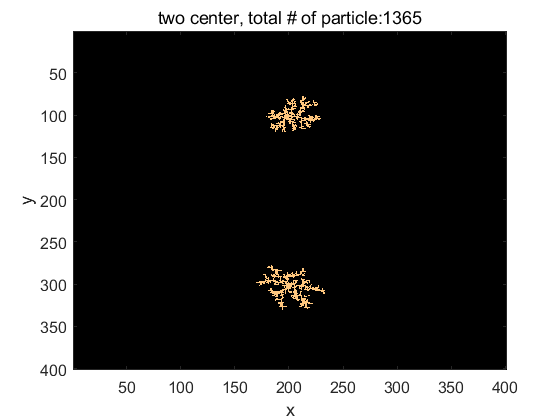
\includegraphics[width=0.45\textwidth]{../result/2_1365}}
		\subfigure[1801 particles(中心相距近)]{
			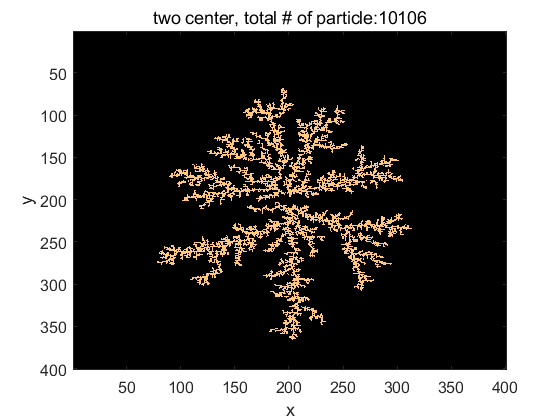
\includegraphics[width=0.45\textwidth]{../result/2_10106}}
		\caption{不同阶段的双中心DLA生长}
	\end{figure}
	
	有趣的是发生了相规避生长的情况,两个团簇不会融合成一个,而是各自占据一半地盘向外延伸。
	
	
	\end{flushleft}
	
	\subsection{分形维数计算}
	
	\subsubsection{sandbox法}
	
	\begin{flushleft}
		先对上述的单中心生长进行计算,采用sandbox法得到结果如下:
		
		$$D=1.679$$	
		
			\begin{figure}[H]
				\centering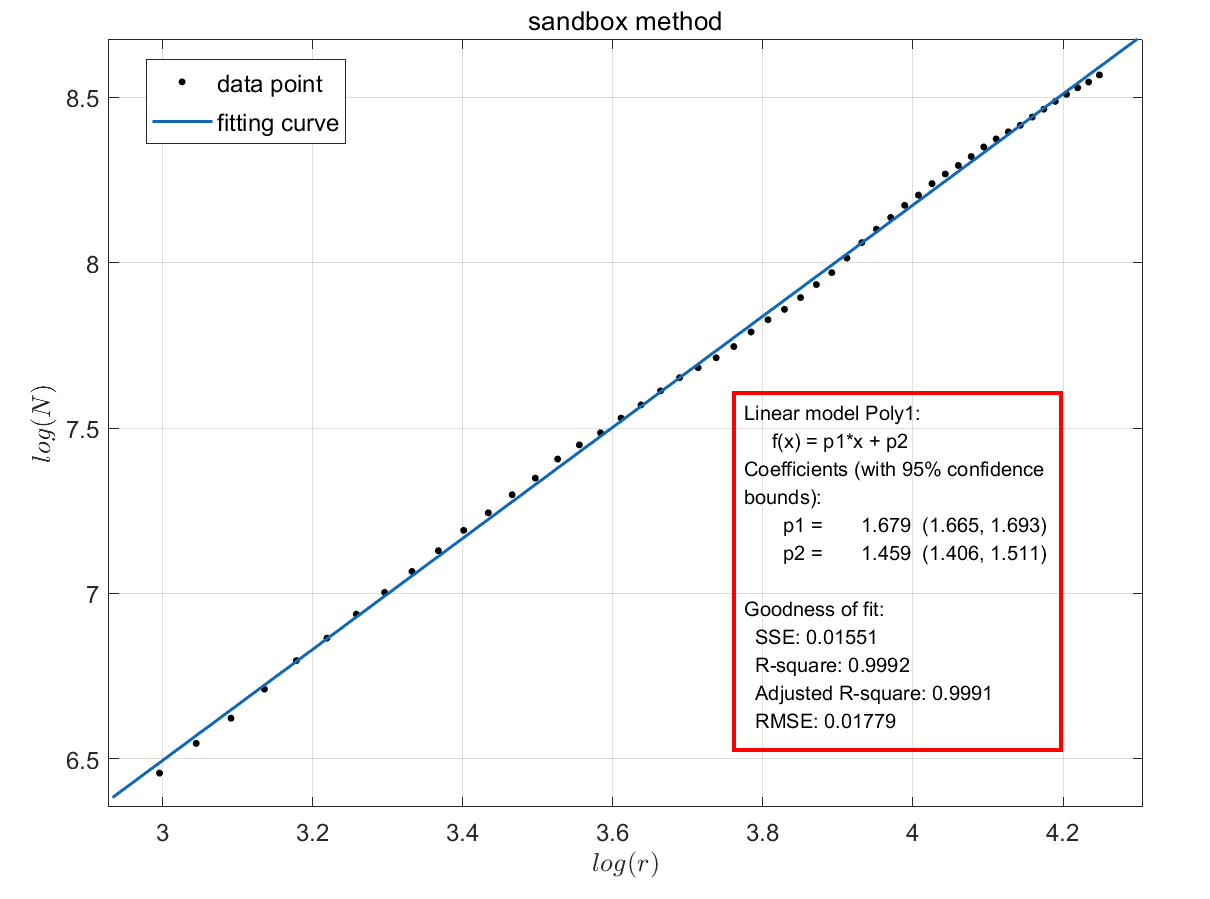
\includegraphics[width=6in]{../result/sandbox}
				\caption{sandbox method}
				\end{figure}
	
		理论上DLA生长的分维数为1.60$\sim$1.70,我们的计算和这个符合。
		
		接着对双中心(图2(b))进行分维数计算:
		
		\begin{figure}[H]
			\centering  %图片全局居中
			\subfigure[原数据]{
				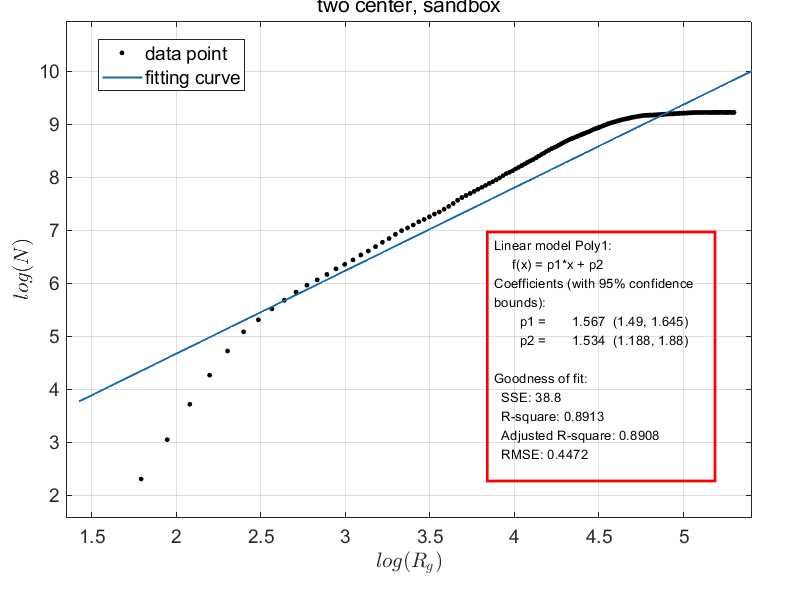
\includegraphics[width=0.45\textwidth]{../result/sandbox_2}}
			\subfigure[舍选处理过]{
				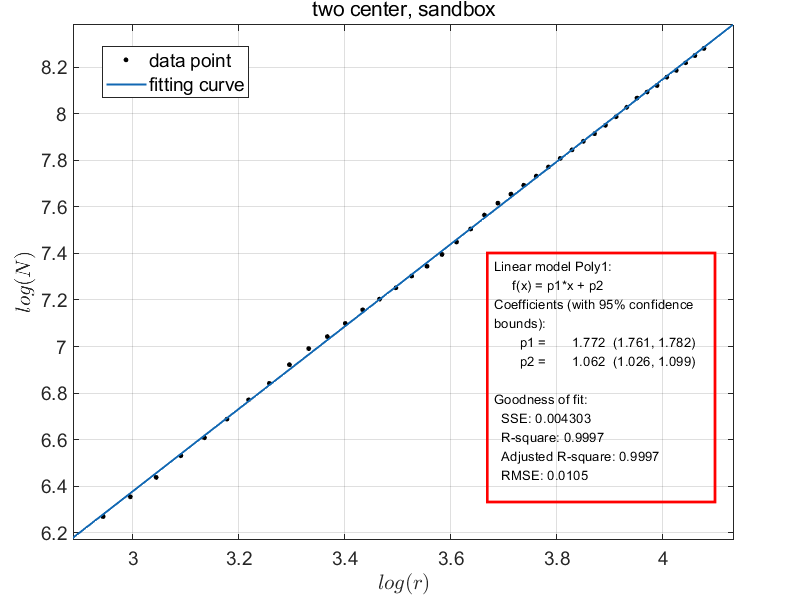
\includegraphics[width=0.45\textwidth]{../result/sandbox_re}}
			\caption{双中心的分维数计算}
		\end{figure}
	
	我此时选择的双中心分别为$cnt[N/2-10][N/2]$和$cnt[N/2+10][N/2]$,所以仍然从$cnt[N/2][N/2]$开始sandbox计数仍然是合理的。只是由于不在是单中心了,线性区域变得更窄了,经过挑选线性区域的图(b)得到的分维数为1.772,略大于理论值,这也一定程度上体现出sandbox法比较适合单中心生长图形。
	
	\subsubsection{回转半径法}
	
	先对上述的单中心生长进行计算,采用回转半径法得到结果如下:
	
	$$D=1.679$$

	这得到的分维数和sandbox法一样,所以说明这个图形分维数约为1.679。
	
	\begin{figure}[H]
		\centering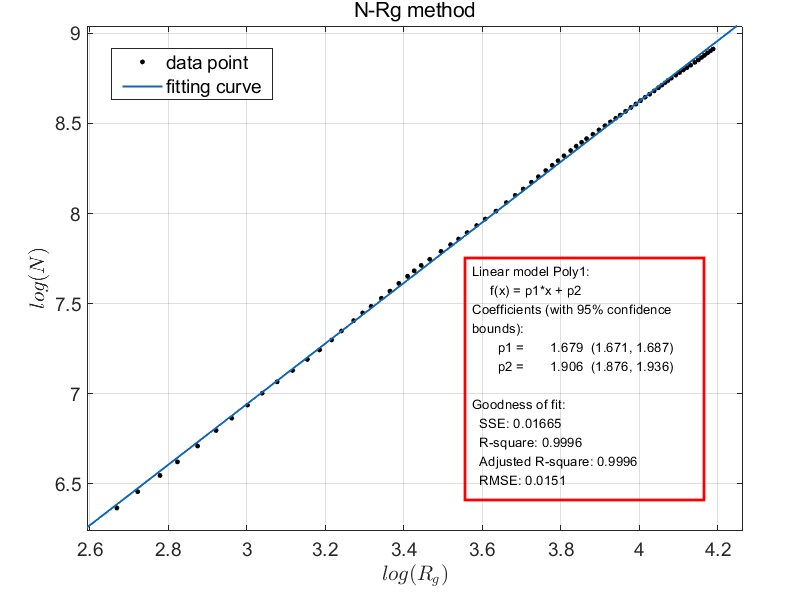
\includegraphics[width=6in]{../result/Rg}
		\caption{$R_g$ method}
	\end{figure}
	
	接着对双中心(图2(b))进行分维数计算:
	
	\begin{figure}[H]
		\centering  %图片全局居中
		\subfigure[原数据]{
			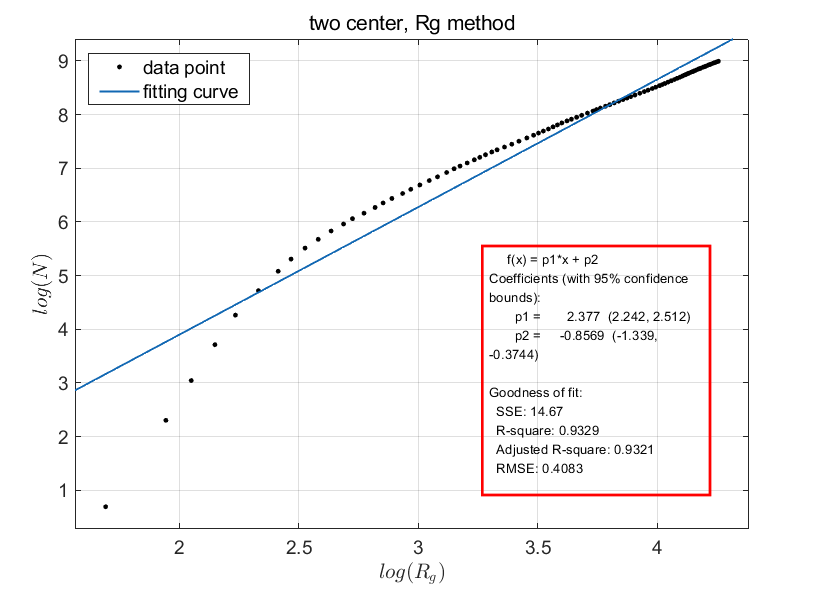
\includegraphics[width=0.45\textwidth]{../result/Rg_2}}
		\subfigure[舍选处理过]{
			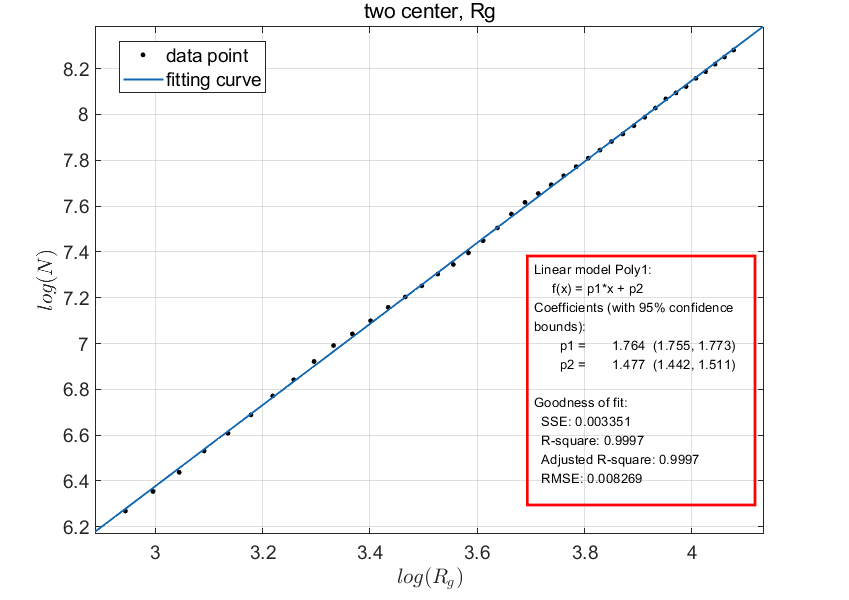
\includegraphics[width=0.45\textwidth]{../result/Rg_re}}
		\caption{双中心的分维数计算}
	\end{figure}
	
	和sandbox法出现类似的偏离线性情形,原因可能是笔者在计算的时候吧$(N/2,N/2)$当成生长中心计算,实际上在多中心时采取下列的公式会更加准确一点:
	
	$$R_g^2=\frac{\sum_{i=1}^N (r_i-r_j)^2}{2N(N-1)}$$
	
	此处计算得到的分维数为:
	
	$$D=1.764$$
	
	略大于理论值范围。
	
		
	\end{flushleft}
	
	
	

%	\begin{figure}[H]
%	\centering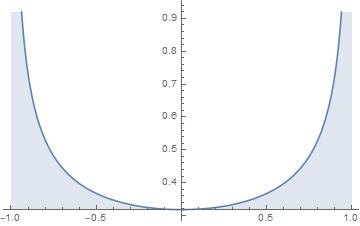
\includegraphics[width=2in]{1.jpg}
%	\caption{something}\label{fig:1}
%	\end{figure}
%		
%	\begin{figure}[H]
%		\centering  %图片全局居中
%		\subfigure[name1]{
%			\label{Fig.sub.1}
%			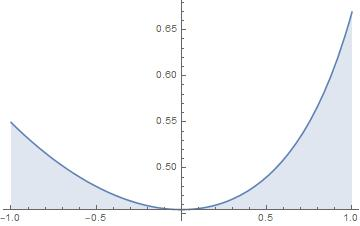
\includegraphics[width=0.45\textwidth]{2.jpg}}
%		\subfigure[name2]{
%			\label{Fig.sub.2}
%			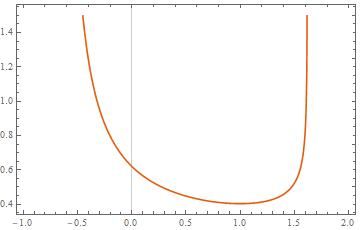
\includegraphics[width=0.45\textwidth]{3.jpg}}
%		\caption{Main name}
%		\label{Fig.main}
%	\end{figure}

	\section{总结}

	
	\begin{itemize}
		
		\item 扩散限制凝聚是一个摸拟薄膜生长,自然沉积过程的很好的模型,具有丰富的物理意义。本次实验通过二维DLA的摸拟,得到了其分维数和基本图形性质,加深了理解。
		
		\item 本次实验采用固定边界,所以最开始生长过程粒子游走到触碰团簇的概率小,需要投入很多粒子,等待时间长。一个比较好的改进方法是将固定边界变成不断变化的生长边界,始终保持比最大团簇尺寸大上数圈,然后以此为边界生长。
		
	\end{itemize}

\end{document}